% TODO maybe introduce weaks and softs??

\chapter{Memory Fundamentals}

Before getting into the details of how to implement your lifetime requirements,
it is important to understand some of what the fundamentals of memory management
in languages like Java. The Java language has a \emph{managed runtime}. In part,
this means that, as a Java program runs, a runtime environment assumes the burden
of key aspects of memory management. This level of management includes as
automatic garbage collection of both instances and Java classes. Therefore, Java
has feature that govern, on your behalf, important aspects of the lifetime of
objects. You need to appreciate what the runtime is doing for you, before
considering how to reshape object lifetimes to better suit your needs.

This chapter introduces the basics of the garbage collector, and how the Java
managed runtime governs object lifetimes. Then, it walks you through the
lifecycle of typical objects from allocation to eventual garbage collection. If
you are comfortable with the basics of memory management, you may discover that
you can skip to the next chapter.

\section{The Garbage Collector}
The \jre decides when the storage allocated to an object should be reclaimed.
This decision is based on a number of criteria. The point of reclamation
depends on the settings you have chosen for various policy knobs, and is also
affected by choices you have made in the application code. However, in most
cases, there is a common structure to the schedule of when objects are
collected.

\paragraph{The Collection Schedule}
Most contemporary garbage collectors deallocate storage in a bulk process 
A language 
when gc runs
In this way, memory consumption over time assumes a sawtooth edge.
\index{Sawtooth Pattern}

\paragraph{Configuration Settings}
You can guide the frequency of 
Xmx and when heap expands
\index{-Xmx command line setting}
\index{-Xms command line setting}

what reclaimed what not

\paragraph{The Nursery, Permspace, and Constant Pools}
\index{Nursery}
\index{Permspace}

\paragraph{Finalizers, and phantom referenes}
\index{Finalization of objects}
\index{Phantom References}

\paragraph{Class Unloading and Lifetime of Statics}

A \code{static} field of an object is one way that Java gives you to indicate
that you want an object to live forever.
\index{Class Unloading}
\index{Static fields}

\paragraph{Concurrent, Parallel, and Real-time Collection}
\index{Concurrent GC}
\index{Parallel GC}
\index{Real-time GC}


\section{The Object Lifecycle}
%Every object created by your application lives for an interval of time from its
%creation to the point that the Java runtime gets around to collecting it. An object's {\em natural} lifetime is defined by the
%interval of time between its first and last necessary use. %cite drag paper
%here?


In a \emph{well-behaved} application, an object's lifetime spans its allocation,
use, and the short period during which the \jre takes control and reclaims the
space. For some subset of an object's actual lifetime, that is the time from
creation to reclamation, your application will make use of the data stored in its
fields. \autoref{fig:typical-lifecycle} illustrates the lifecycle of a typical
object in a well behaved application.

\begin{figure}
	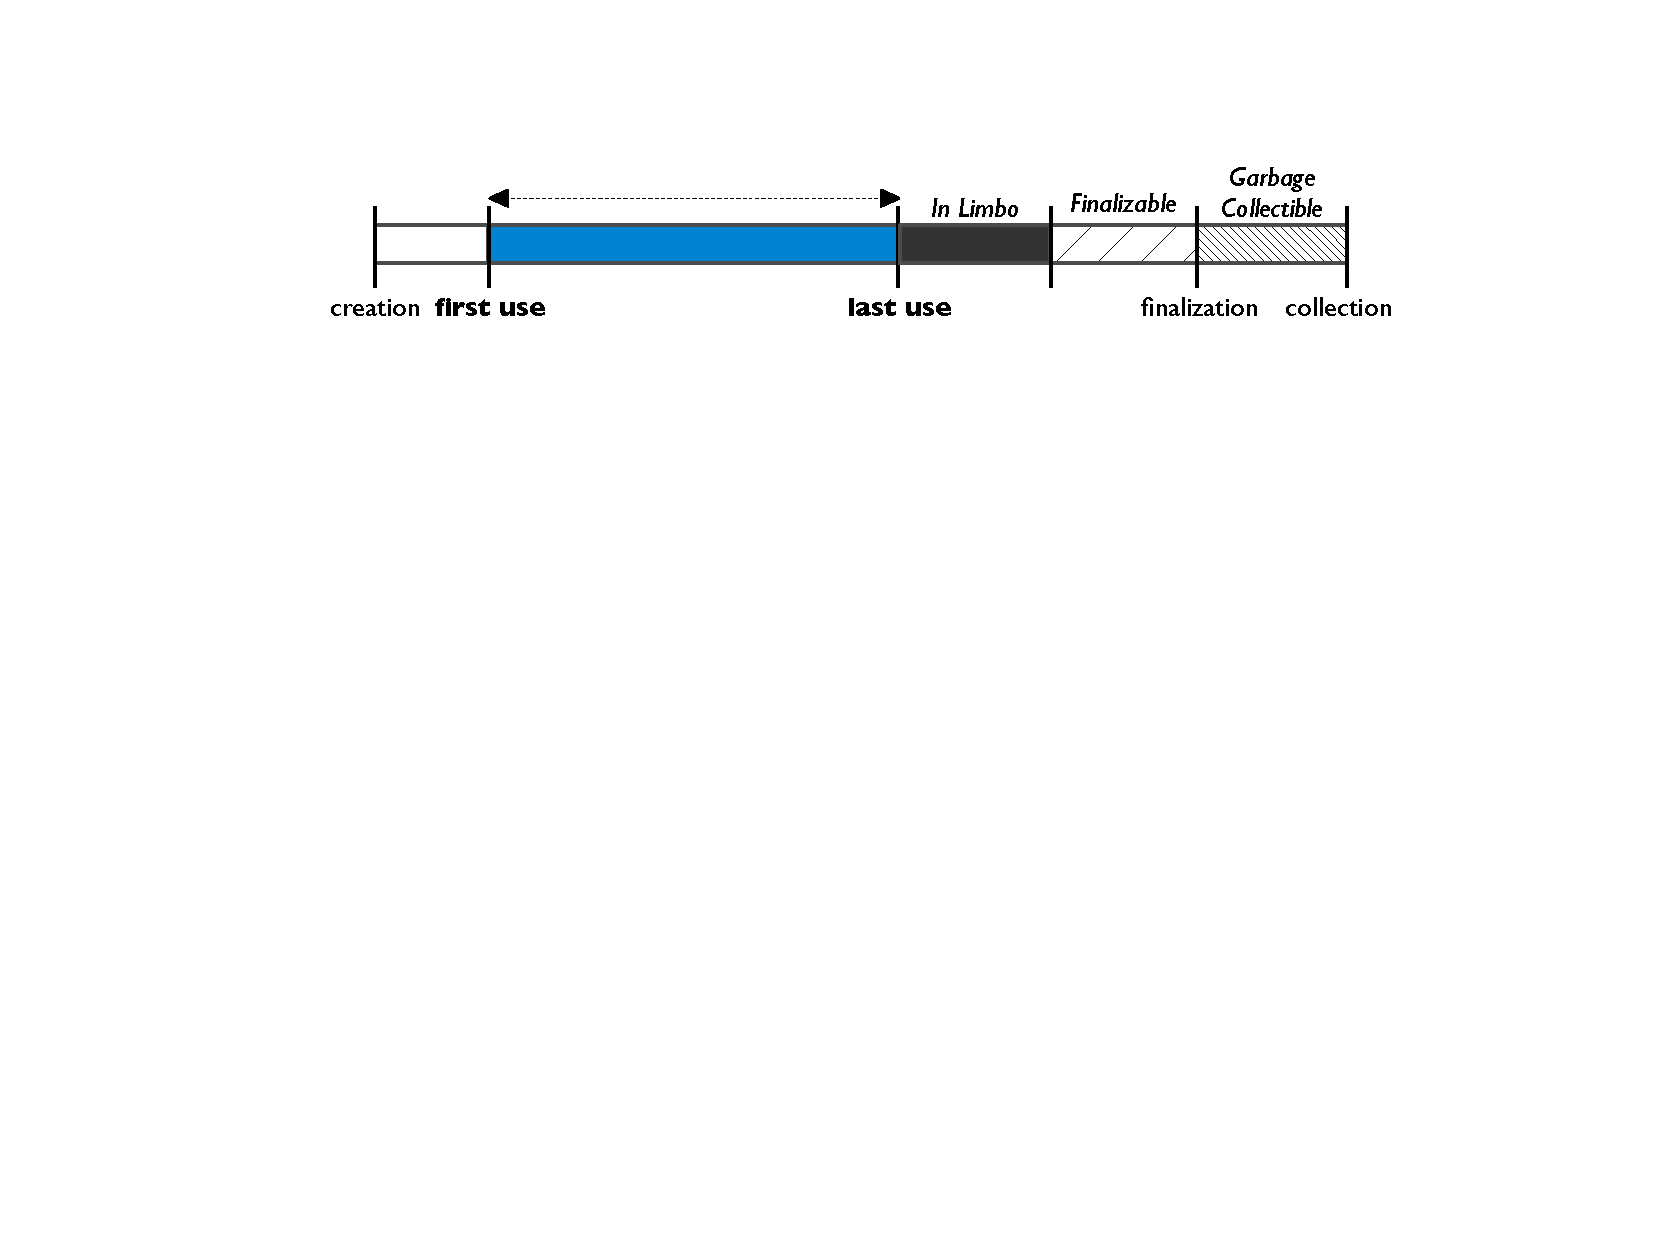
\includegraphics[width=0.9\textwidth]{part4/Figures/lifetime/object-lifecycle}
	\caption{Timeline of the life of an object.}
	\label{fig:typical-lifecycle}
\end{figure}

\begin{example}{Parsing a Date} Consider a loop that shows an easy way to parse
a list of dates. What objects are created, and what are their lifetimes?
\begin{shortlisting}
for (String string : inputList) {
	ParsePosition pos = new ParsePosition(0);
	SimpleDateFormat parser = new SimpleDateFormat();
	System.out.println(parser.parse(string, pos));
}
\end{shortlisting}
\end{example}

For each iteration of this loop, this code takes a date that is represented as a
string and produces a standard Java \class{Date} object. In doing so, a number of
objects are created. Two of these are easy to see, in the two \code{new} calls
that create the parse position and date parser objects. The programmer who wrote
this created two objects, but many more are created by the standard libraries to
finish the task. These include a calendar object, number of arrays, and the
\class{Date} itself. None of these objects are used beyond the iteration of the
loop in which they were created. Within one iteration, they are created, almost
immediately used, and then enter a state of \emph{limbo}.

\callout{limbo}{Objects in Limbo}{
\index{Limbo}
In limbo, an object will never be used again, or at least not for long time,
but the \jre doesn't yet know that this is the case. The object hangs
around, taking up space in the Java heap until the point when it exits limbo.}

The \code{pos} object represents to the parser the position within the
input string to begin parsing. The implementation of the \code{parse} method
uses it early on in the process of parsing. Despite being unused for the
remainder of the parsing, the \jre does not know this until the current
iteration of the loop has finished. This time in limbo also includes the
entirety of the call to \code{System.out.println}, an operation entirely
unrelated to the creation or use of the parse position object. Once the current
loop iteration finishes, these two objects will exit limbo, and become garbage
collectible.\index{Exiting Limbo}

\begin{figure}
	\centering
	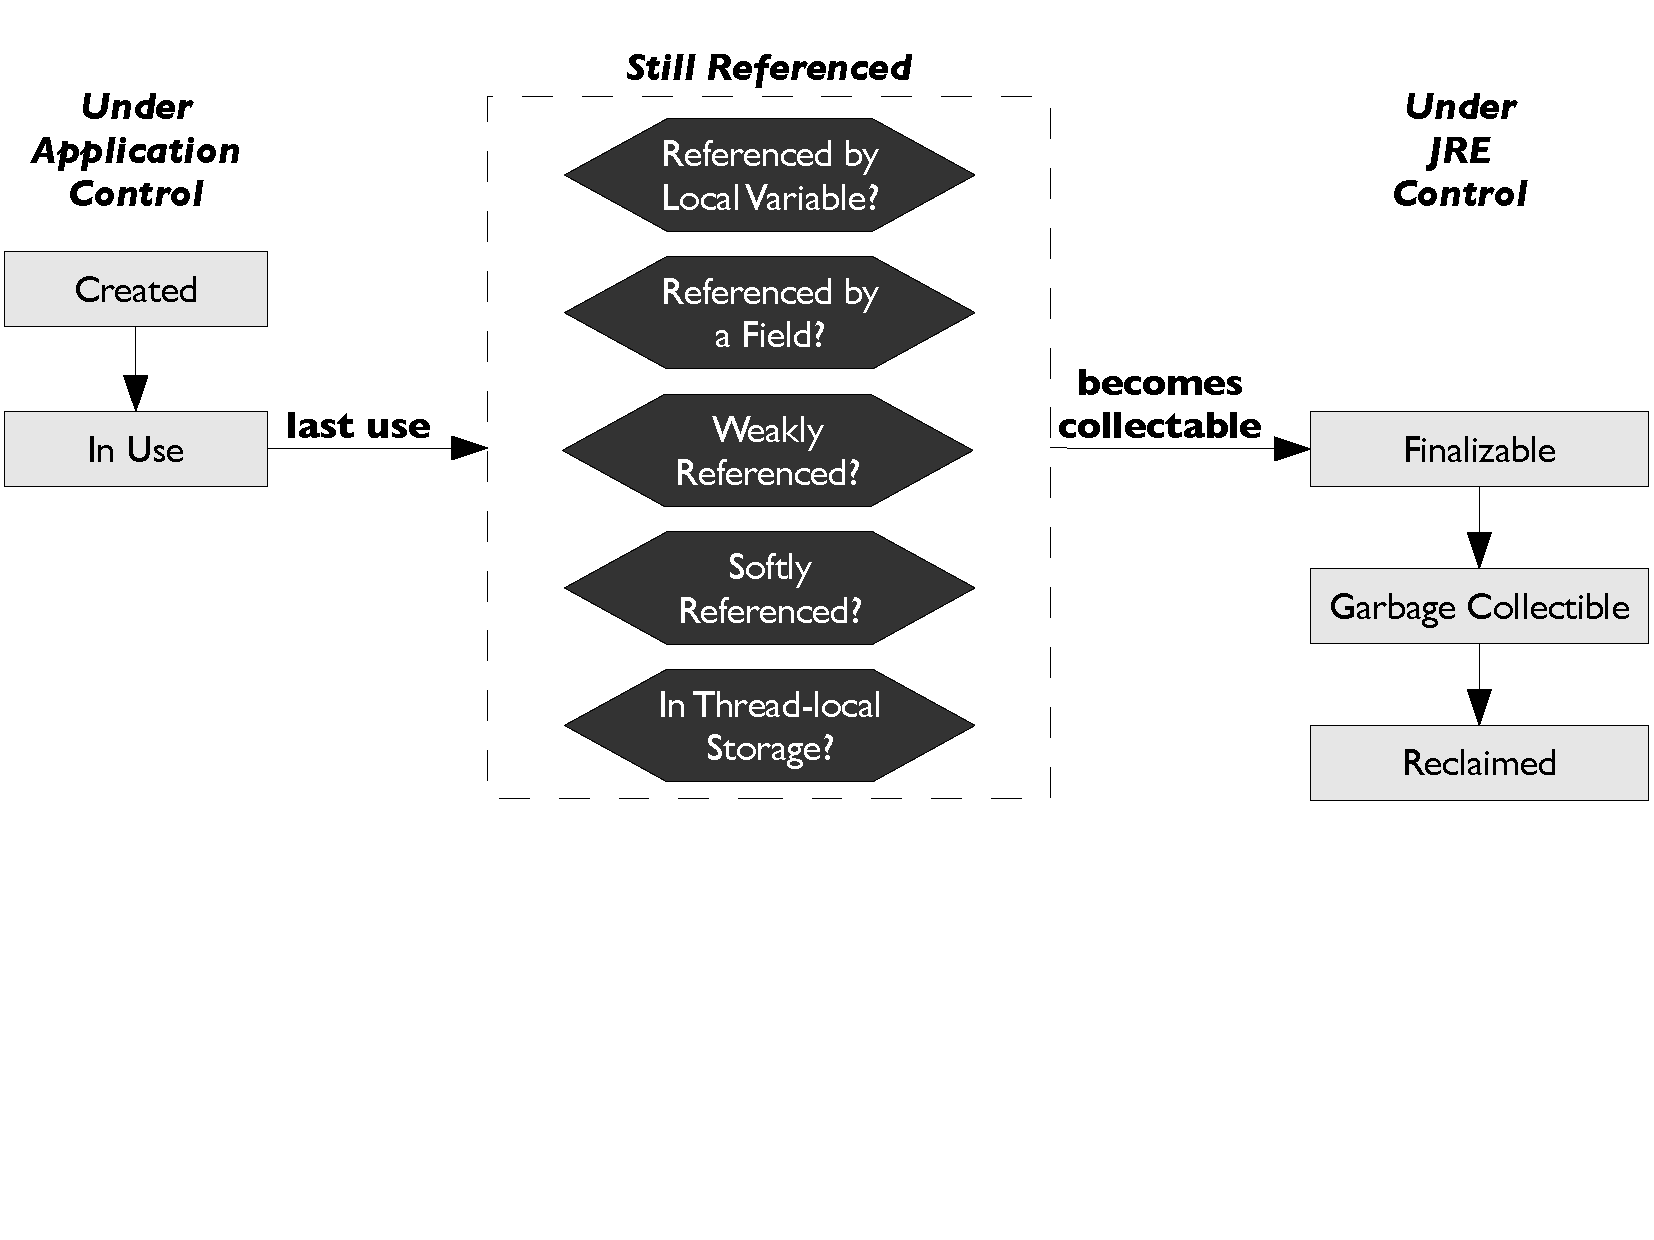
\includegraphics[width=\textwidth]{part4/Figures/lifetime/states}
	\caption{After its last use, an object enters a kind of limbo: the application
	is done with it, but the \jre hasn't yet inferred this to be the case. When an
	object exits limbo depends on the way it is referenced.}
		\label{fig:limbo-exit}
\end{figure}


\begin{comment}
\begin{figure}
	\centering
	\subfigure[The lifecycle of a typical object and its data.]{
	\label{fig:typical-lifecycle1}
			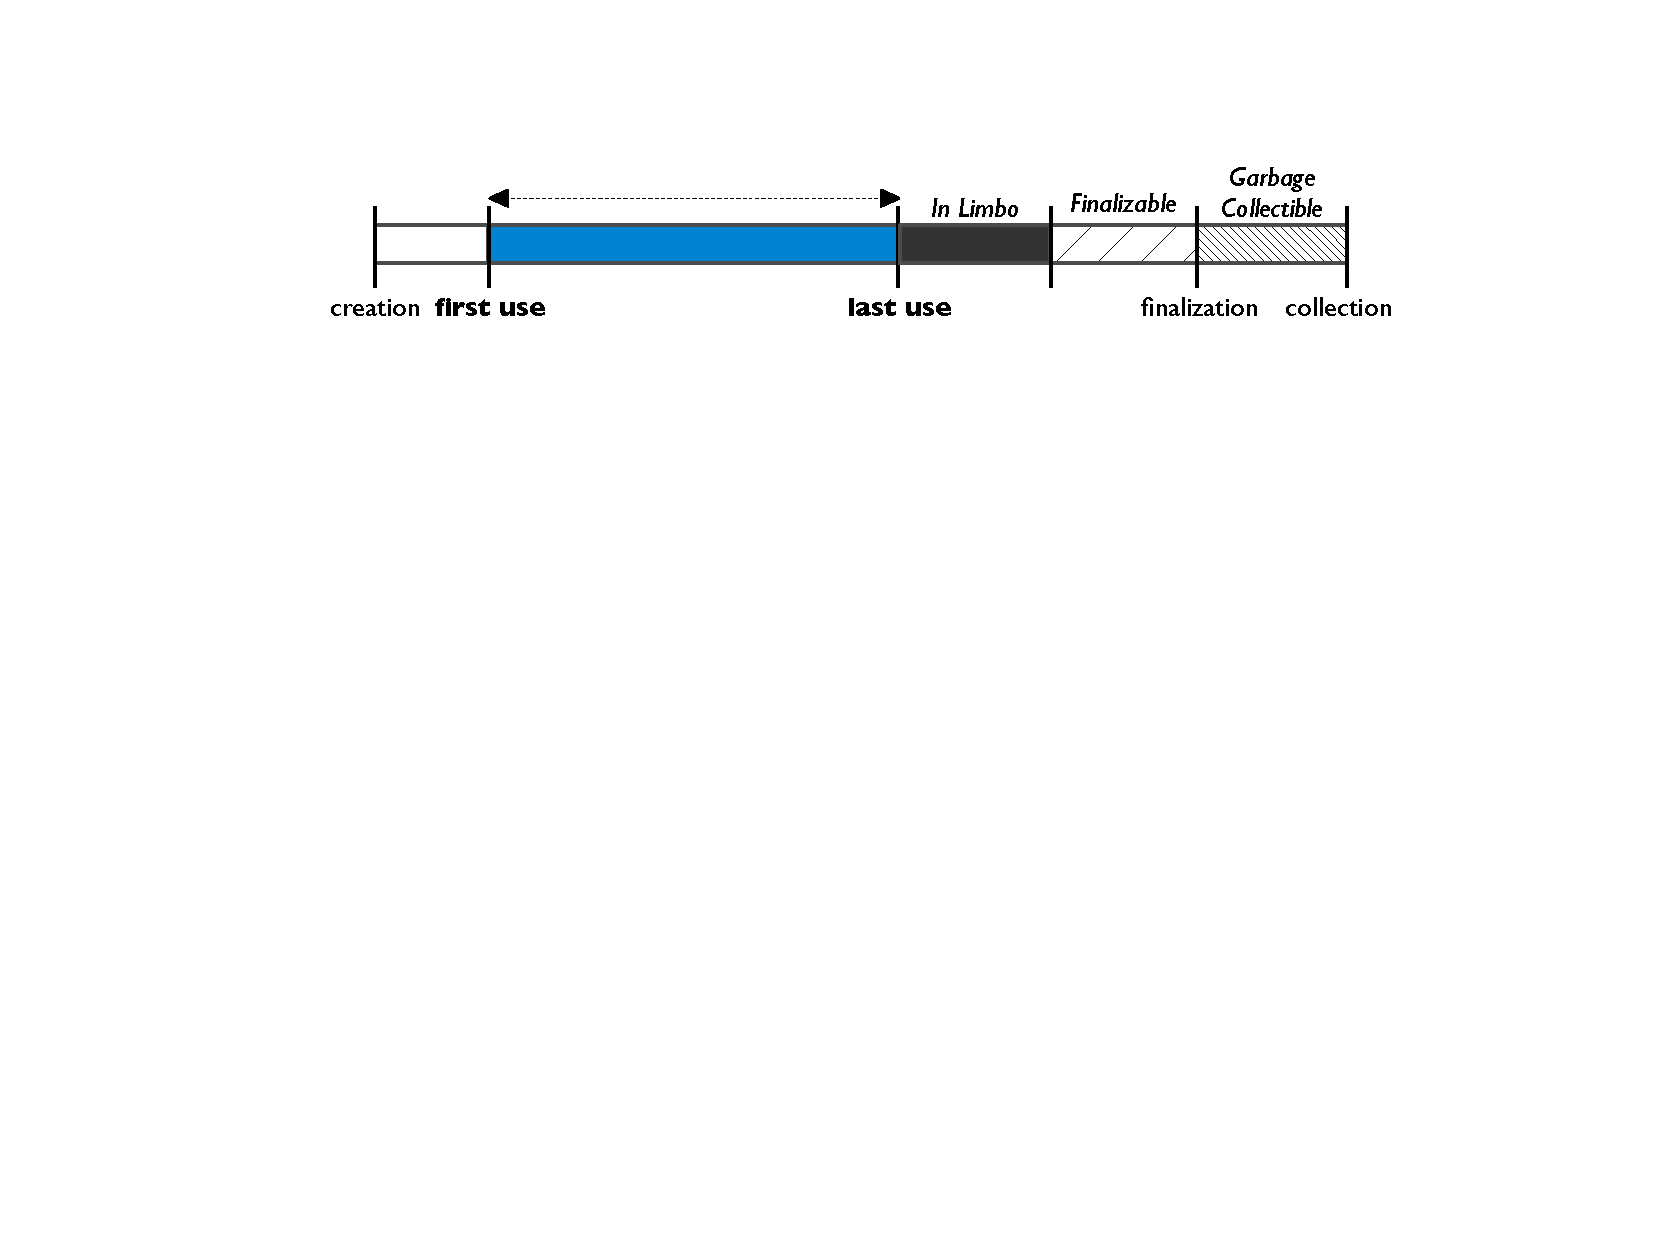
\includegraphics[width=0.95\textwidth]{part4/Figures/lifetime/object-lifecycle}
	}
	\subfigure[A situation where there are long periods between uses of an
	object's data.]{
	\label{fig:typical-lifecycle2}
		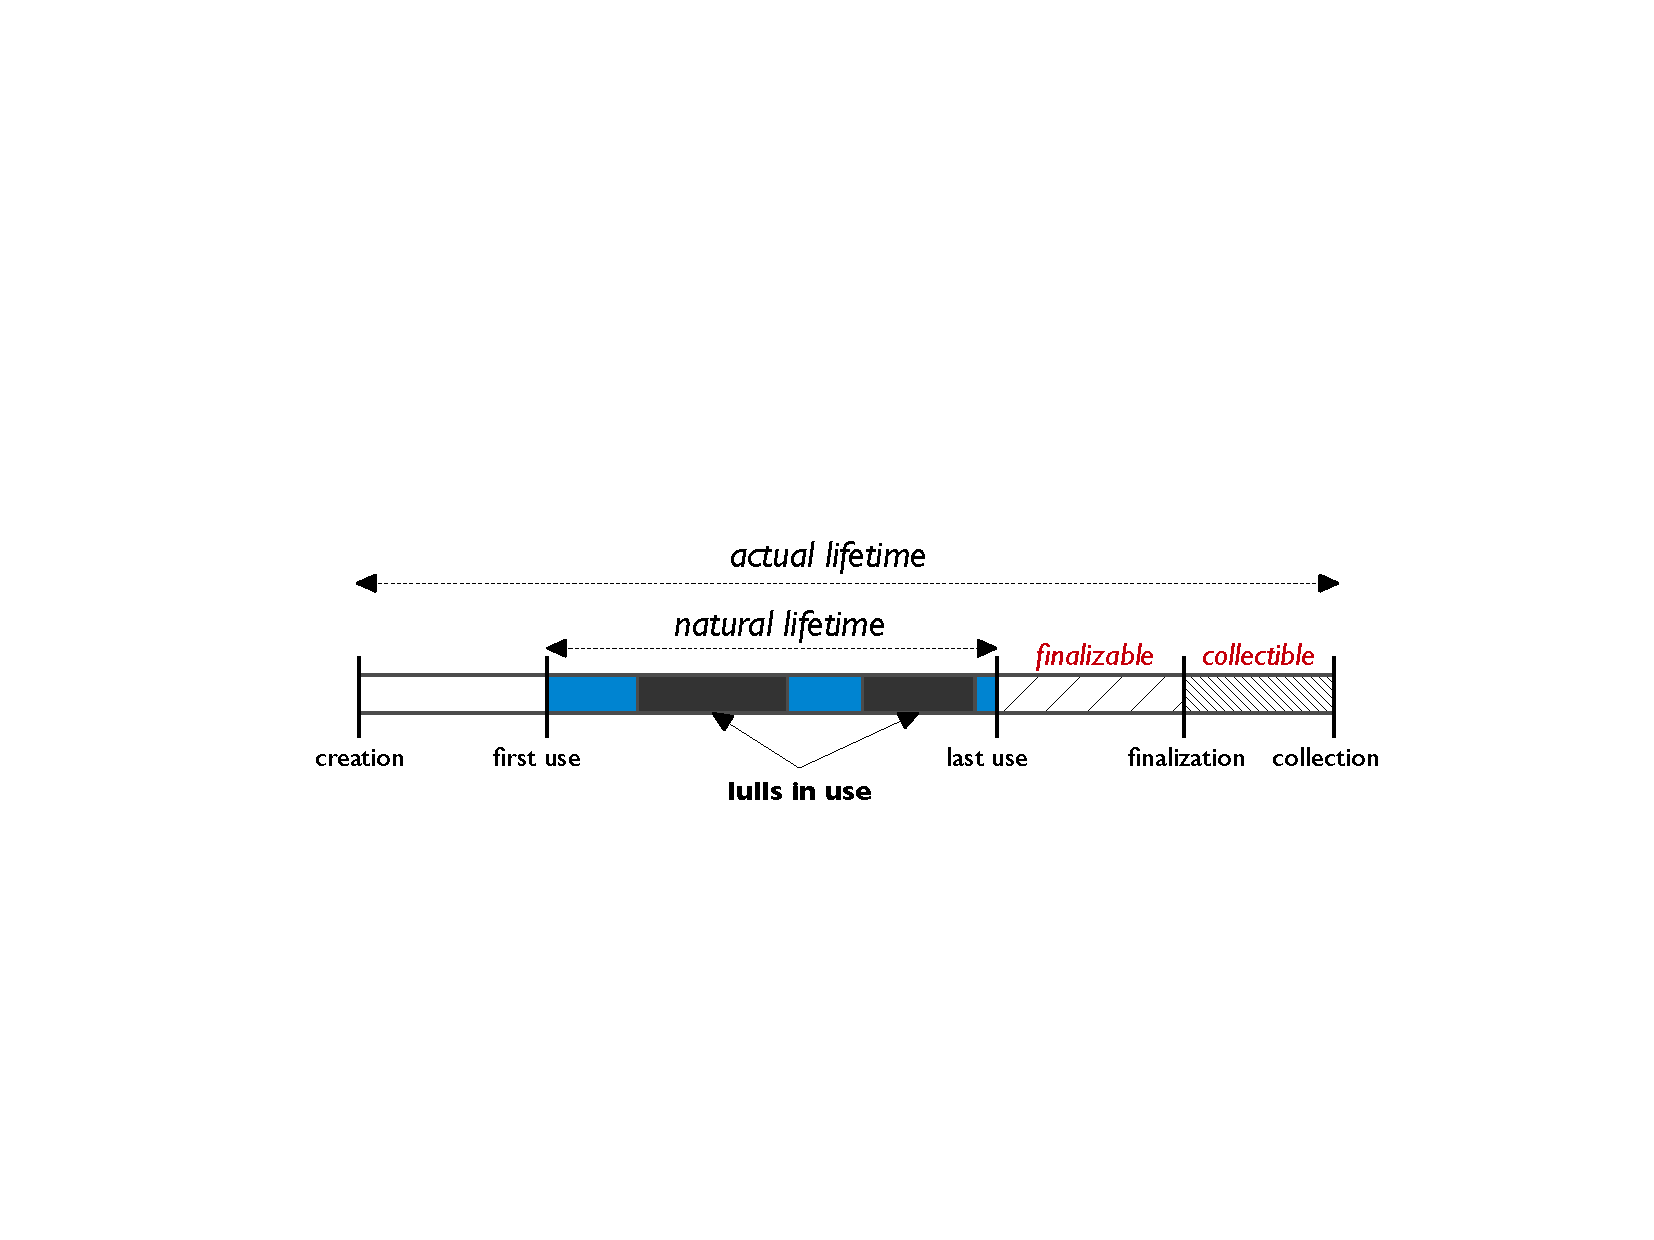
\includegraphics[width=0.95\textwidth]{part4/Figures/lifetime/object-lifecycle-lulls}
	}
	\subfigure[The lifecycle of the data  that is loaded from
	disk three times, and the objects that store it.]{
	\label{fig:typical-lifecycle3}
		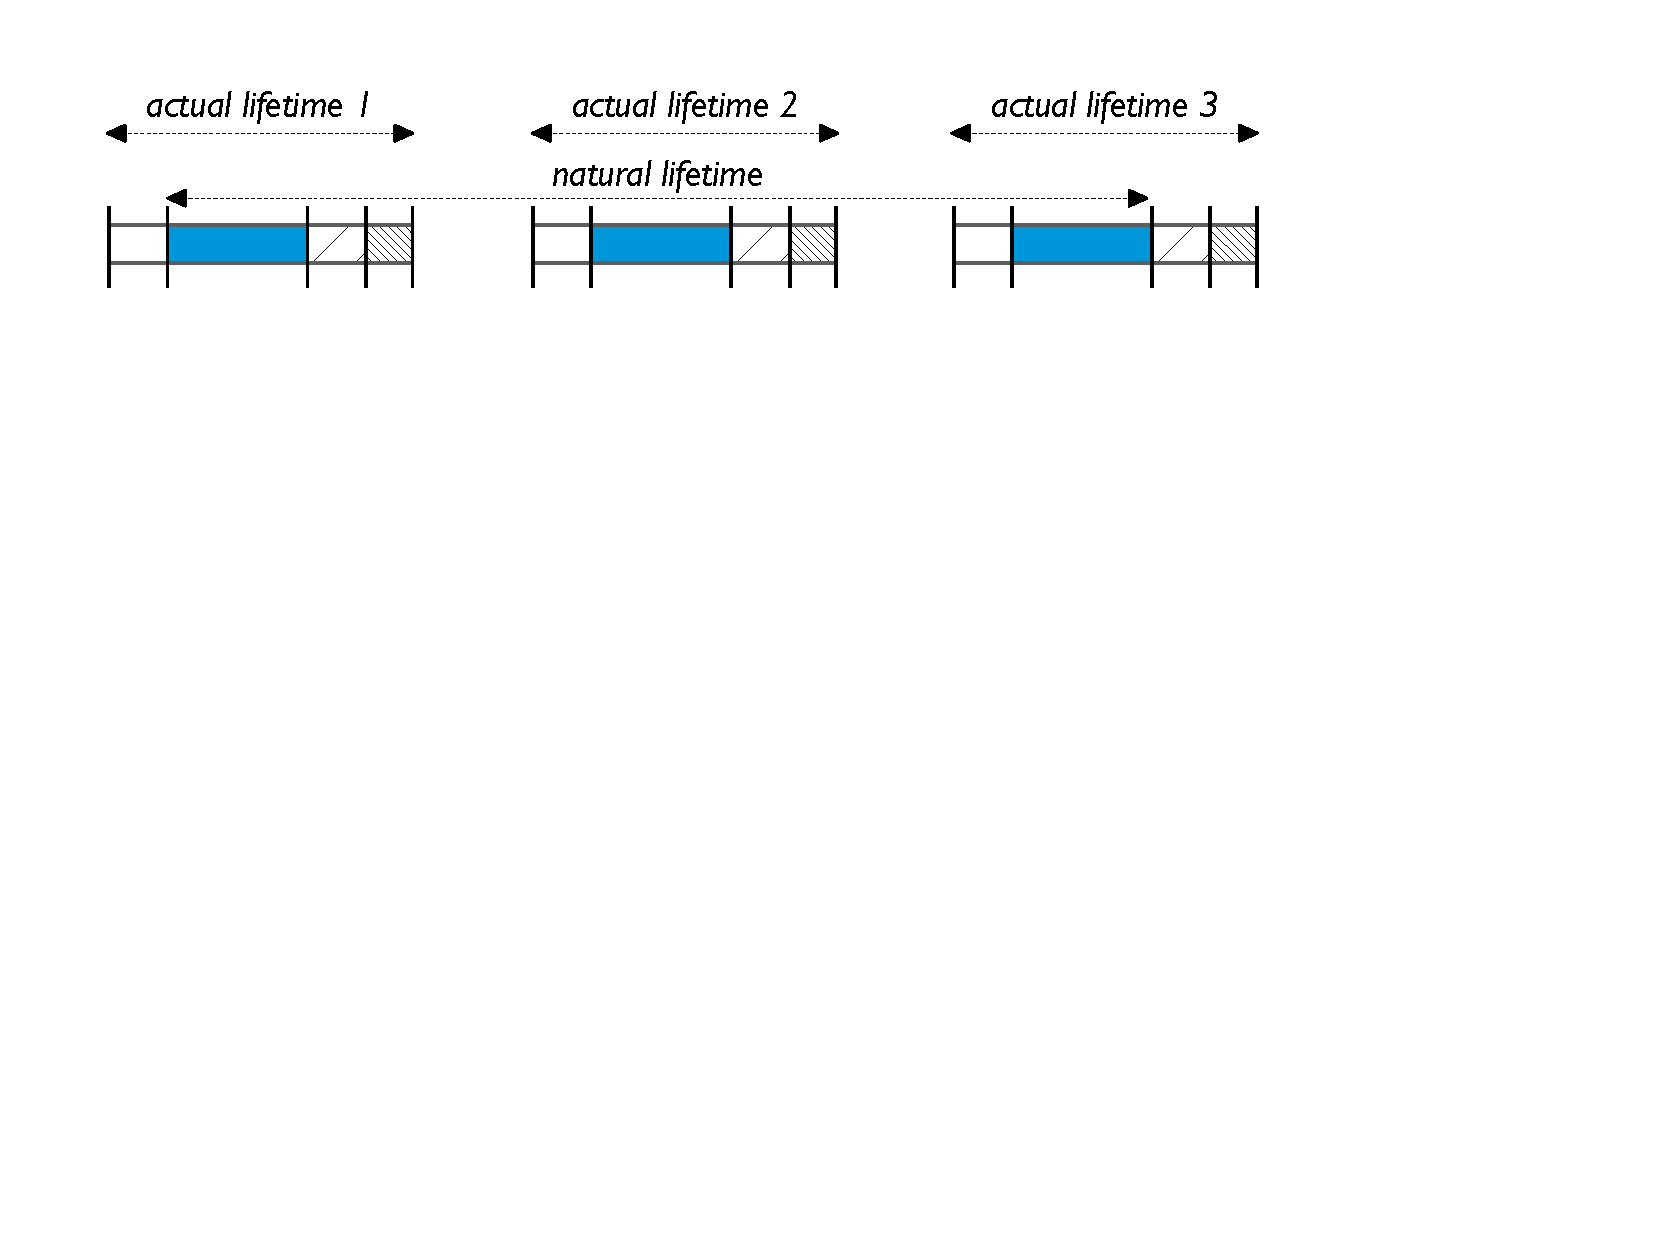
\includegraphics[width=0.9\textwidth]{part4/Figures/object-lifecycle2}
	}
	\caption{Examples of Natural and Actual lifetimes.}
	\label{fig:typical-lifecycle}
\end{figure}
\end{comment}


